\documentclass[a2paper, 12pt]{article}
\usepackage[font={huge, bf}]{caption}
\usepackage{fontspec}
\setmainfont{Arial}
\usepackage{subcaption}
\usepackage{graphicx}
\usepackage{tikz}
\usepackage{tikzsymbols}
\usetikzlibrary{calc,patterns,shapes.geometric}
\usepackage{float}
\usepackage{pdflscape}
\usepackage{geometry}
\geometry{landscape, margin=2cm}
\captionsetup[subfigure]{justification=justified,singlelinecheck=false}
\pagestyle{empty}

\def\centerarc[#1](#2)(#3:#4:#5){\draw[#1] ($(#2)+({#5*cos(#3)},{#5*sin(#3)})$) arc (#3:#4:#5);}

\begin{document}
	\vspace*{\fill}
	\begin{figure}[!htbp]
		\centering
		\begin{subfigure}[b]{0.48\textwidth}
			\caption{Figure 1}
			\centering
			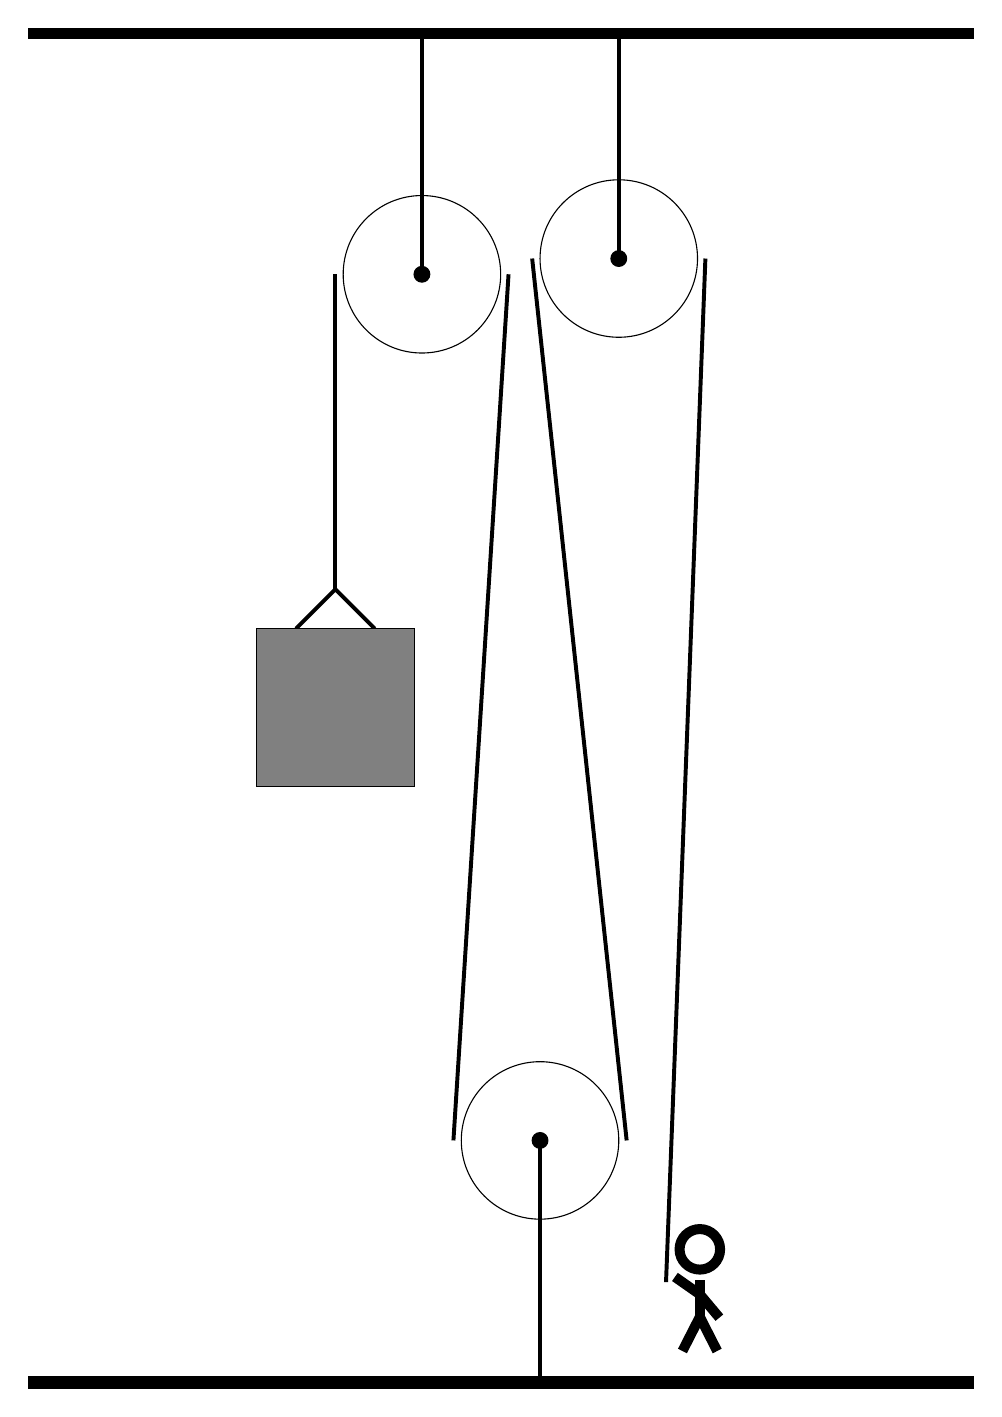
\begin{tikzpicture}
				\draw[fill=black] (-4, 14) rectangle (8, 14.125);
				
				\draw (1, 11) circle (1);
				\draw[fill=black] (1, 11) circle (0.1);
				\draw[line width=0.5mm]  (1, 14) -- (1, 11);
				
				\draw[fill=white](2.5, 0) circle (1);
				\draw[fill=black] (2.5, 0) circle (0.1);
				\draw[line width=0.5mm]  (2.5, -3) -- (2.5, 0);
				
				\draw[fill=white](3.5, 11.2) circle (1);
				\draw[fill=black] (3.5, 11.2) circle (0.1);
				\draw[line width=0.5mm] (3.5, 14) -- (3.5, 11.2);
				
				\draw[line width=0.5mm] (-0.6, 6.5) -- (-0.1, 7.0) -- (0.4, 6.5);
				\draw[fill=black!50] (-1.1, 6.5) rectangle (0.9, 4.5);
				
				\draw[line width=0.5mm] (-0.1, 11) -- (-0.1, 7.0);
				\centerarc[line width=0.5mm](1, 11)(0:180:1.1);
				\draw[line width=0.5mm](2.1, 11) -- (1.4, 0);
				\centerarc[line width=0.5mm](2.5, 0)(180:360:1.1);
				\draw[line width=0.5mm](3.6, 0) -- (2.4, 11.2);
				\centerarc[line width=0.5mm](3.5, 11.2)(0:180:1.1);
				\draw[line width=0.5mm](4.6, 11.2) -- (4.1, -1.8);
				
				\node at (4.5, -1.9) {\scriptsize \Strichmaxerl[10][-35][-50]};
				
				\draw[fill=black] (-4, -3) rectangle (8, -3.15);
			\end{tikzpicture}
		\end{subfigure}
		\hfill
		\begin{subfigure}[b]{0.48\textwidth}
			\caption{Figure 2}
			\centering
			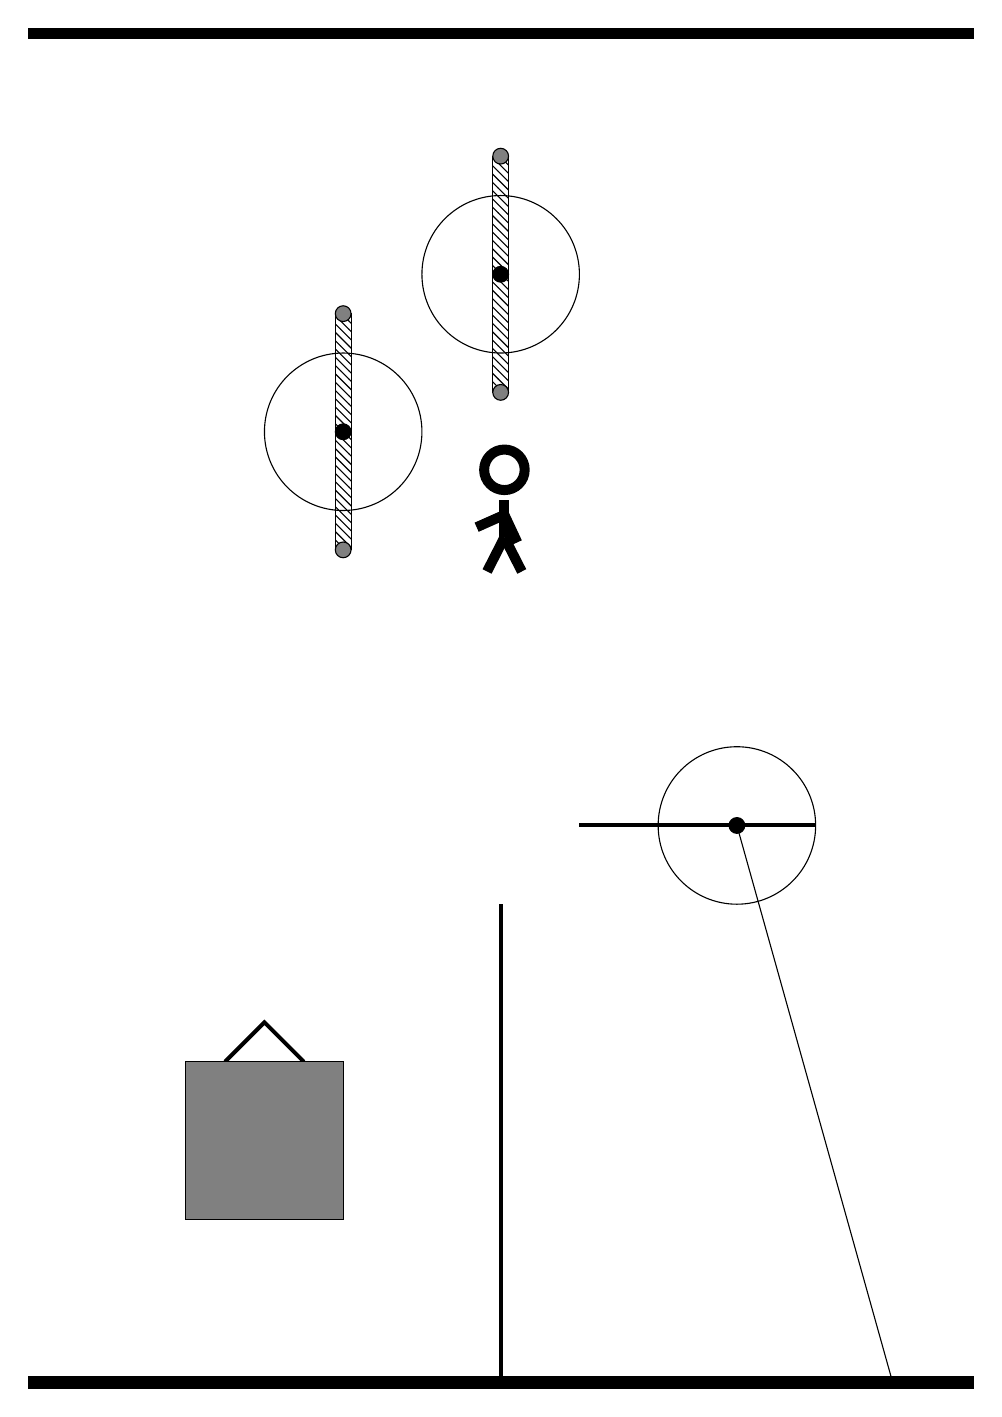
\begin{tikzpicture}
				\draw[fill=black] (-4, 14) rectangle (8, 14.125);
				
				\draw (2,11) circle (1);
				\draw[fill=black] (2,11) circle (0.1);
				\draw[pattern=north west lines, pattern color=black] (1.9,12.5) rectangle (2.1,9.5);
				\draw[fill=black!50] (2,12.5) circle (0.1);
				\draw[fill=black!50] (2,9.5) circle (0.1);
				
				\draw (5,4) circle (1);
				\draw[fill=black] (5,4) circle (0.1);
				\draw (7,-3.15) -- (5,4);
				
				\draw (0,9) circle (1);
				\draw[fill=black] (0,9) circle (0.1);
				\draw[pattern=north west lines, pattern color=black] (-0.1,10.5) rectangle (0.1,7.5);
				\draw[fill=black!50] (0,10.5) circle (0.1);
				\draw[fill=black!50] (0,7.5) circle (0.1);
				
				\draw[line width=0.5mm](-1.5,1) --  (-1,1.5) -- (-0.5,1);
				\draw[fill=black!50] (-2, 1) rectangle (0, -1);
				
				\draw[line width = 0.5mm] (3,4) -- (6,4);
				\centerarc[line width = 0.5mm](3,3)(90:180:1);
				\draw[line width = 0.5mm] (2,3) -- (2,-3);
				
				\node at (2, 8) {\scriptsize \Strichmaxerl[10][115][-156]};
				
				\draw[fill=black] (-4, -3) rectangle (8, -3.15);
			\end{tikzpicture}
		\end{subfigure}
	\end{figure}
		\vspace*{\fill}
\end{document}